\documentclass{article}
\usepackage{packages}
\usepackage[utf8]{inputenc}
\usepackage[T1]{fontenc}
\usetikzlibrary{shapes.geometric}

\newcommand{\ve}[1]{\mathbf{#1}}

\begin{document}

\section*{Module I}

\begin{figure}[ht]

\begin{minipage}{0.5\textwidth}
	\centering
	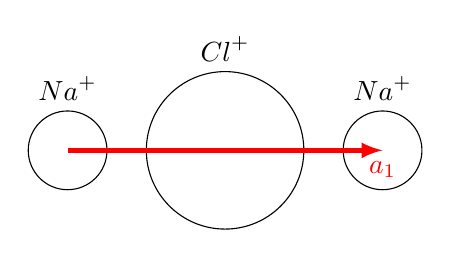
\begin{tikzpicture}
        \node (circle1) [draw, circle, minimum size = 1cm] at (0, 0) {};
        \node (circle2) [draw, circle, minimum size = 2cm] at (2, 0) {};
        \node (circle3) [draw, circle, minimum size = 1cm] at (4, 0) {};
        \draw [ultra thick, -latex, red] (0, 0) -- (4,0) node [below] {$a_1$};
        \node[above] at (circle1.north) {$\text{Na}^+$};
        \node[above] at (circle2.north) {$\text{Cl}^+$};
        \node[above] at (circle3.north) {$\text{Na}^+$};
	\end{tikzpicture}
	\caption{Basis vector of the $\text{NaCl}$ 1D lattice}
	\label{fig:1DNaCl}
\end{minipage}
\begin{minipage}{0.5\textwidth}
    \centering
	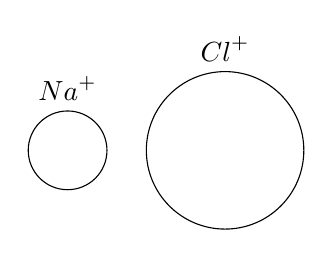
\begin{tikzpicture} 
        \node (circle1) [draw, circle, minimum size = 1cm] at (0, 0) {};
        \node (circle2) [draw, circle, minimum size = 2cm] at (2, 0) {};
        \node[above] at (circle1.north) {$\text{Na}^+$};
        \node[above] at (circle2.north) {$\text{Cl}^+$};
    \end{tikzpicture}
    \caption{Unit cell of the $\text{NaCl}$ 1D lattice}
\end{minipage}
\end{figure}

\subsection*{Exercise 1}

\subsubsection*{(a)}
The basis vector is a vector that starts from an atom and goes to the closer atom of the same type. For example we can choose the leftmost $\text{Na}^+$ as the origin and we draw a vector until the second $\text{Na}^+$. The base unit cell is made of a couple $\text{Na}^+ + \text{Cl}^-$.

\subsubsection*{(b)}
Let us take a $\text{Na}^+$ atom at position x and suppose that the chain is infinitely long both at the left and at the right. Each $\text{Cl}^-$ atom exerts an attractive force (negative potential) on the $\text{Na}^+$ atom and each other $\text{Na}^+$ exerts a repulsive one (positive potential). Hence, in atomic units
$$V(x) = 2 \cdot \left[\frac{1}{a} - \frac{1}{2a} + \frac{1}{3a} - \dots \right]= \frac{2}{a }\sum_{n=1}^{+\infty} \frac{(-1)^{n+1}}{n} = \frac{2 \ln 2}{a}$$
where $a$ is the interatomic distance between two atoms. The Madelung constant is $M = 2 \ln 2$ 

\subsubsection*{(c)}
A consequence of the presence of only a finite number of atoms is that symmetry is broken: each atom has now a different number of atoms on its right and left (except for the central one) and this 
effect becomes smaller as the number of atoms increases (more atoms can be approximated as "centrals"). Remember that the Madelung constant is a geometrical factor related to the energy per molecule in the crystal. 
One can now proceed in two different ways which will be equivalent in the limit of large $N$ as shown in figure \ref{fig:Madelung_constant_Natoms}.
\begin{enumerate}
    \item Neglect border effects and consider each atom as "central". This can be reasonable since the Coulomb potential decreases rapidly with the atom index. In this case the total energy of the lattice is approximately
    $U = NU_i$ where
    $$ U_i = 2\sum_{n=1}^{N/2}\frac{(-1)^n}{n a} = \frac{\alpha}{a}$$
    and $\alpha$ is the Madelung constant.
    \item Consider the border effects and the fact that not all atoms have the same energy. In this case the value of the Madelung constant would depend on the chosen atom, so we calculate an "average" Madelung constant by calculating the average energy of each molecule in the crystal as $V_{tot}/N_{molecules} = V_{tot}/(N/2)$ and use that expression to evaluate the Madelung constant. \\
        The total energy of the system can be computed as a sum over all the particles' interactions. If we begin the chain with a $\text{Na}^+$ atom ($n=0$), the charge of the $n-th$ atom in the chain is in atomic units $(-1)^n$, hence
        $$U = \frac{1}{2} \sum_{i \neq j} \frac{(-1)^i(-1)^j}{r_{ij}} = \frac{1}{2} \sum_{i \neq j} \frac{(-1)^{i+j}}{|i-j| \, a} =
        \frac{N\alpha}{2a}$$
        and this provides an estimation for the Madelung constant $\alpha$.
\end{enumerate} 
The Madelung constant for both models as a function of the number of atoms is plotted in figure \ref{fig:Madelung_constant_Natoms}.
\begin{figure}[h]
    \centering 
    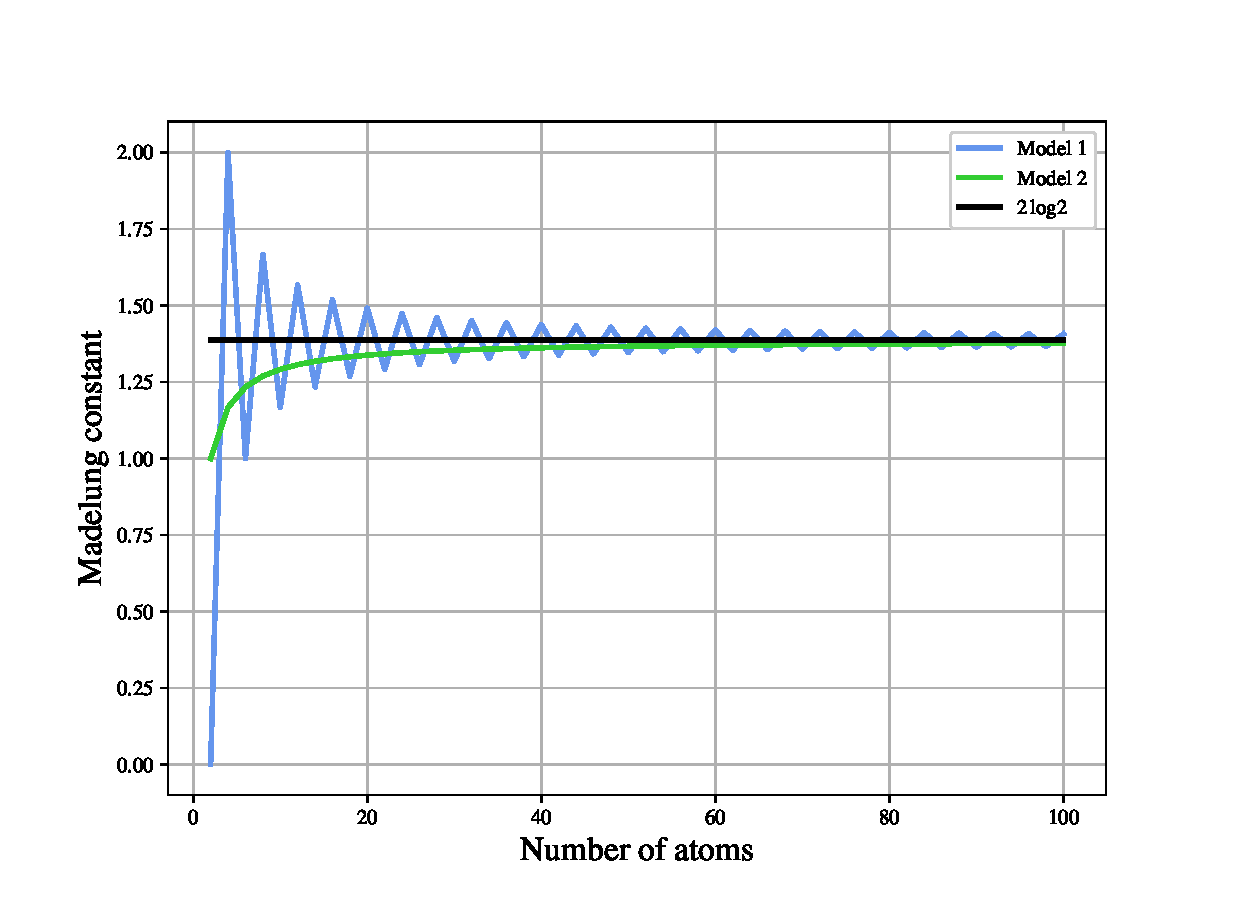
\includegraphics[scale=0.7]{figures/madelung.eps}
    \caption{Madelung constant as a function of the number of atoms. The first model consider each atom as central hence assigning to each atom the same energy. The second model considers the fact that for finite $N$ atoms have
    differen energies and }
    \label{fig:Madelung_constant_Natoms}
\end{figure}

\subsubsection*{(d)}
To simplify the calculations we here neglect border effects and calculate the energy of the crystal as the sum of the electrostatic energy and the Pauli repulsion energy (nearest neighbour only). Let us denote with $a$ the interatomic distance of the lattice. Each atom in the center of the crystal has energy equal to
\begin{equation*}
    U_i(a) = 2 \sum_{i \neq j}U_{ij}(a) = 2\left(\lambda e^{-a/\rho} - \sum_{i \neq j}\frac{1}{r_{ij}}\right) = 
    2\left(\lambda e^{-a/\rho} - \sum_{n=1}^{N/2}\frac{(-1)^{n}}{n}\right)
\end{equation*}
The equilibrium distance can be obtained by searching the minimum of the energy per atom
\begin{equation*}
    \frac{\partial U_i}{\partial a} = 0 \quad \longrightarrow \quad a^2\exp(-a/\rho) = \frac{\rho \alpha}{2\lambda}
\end{equation*}
The equation can be solved numerically and the the result is reported in figure \ref{fig:NaCl_constant}. In addition we can use this 
expression to rewrite the crystal energy as 
\begin{equation*}
    U_{tot} = -\frac{N\alpha}{R_0} \left(1-\frac{\rho}{a}\right)
\end{equation*}

Figure \ref{fig:crystal_energy} reports the energy of the crystal as a function of the number of atoms and figure \ref{fig:energy_per_atom} reports the lattice energy divided by the number of atoms.
\begin{figure}
\begin{minipage}{.5\textwidth}
    \centering
    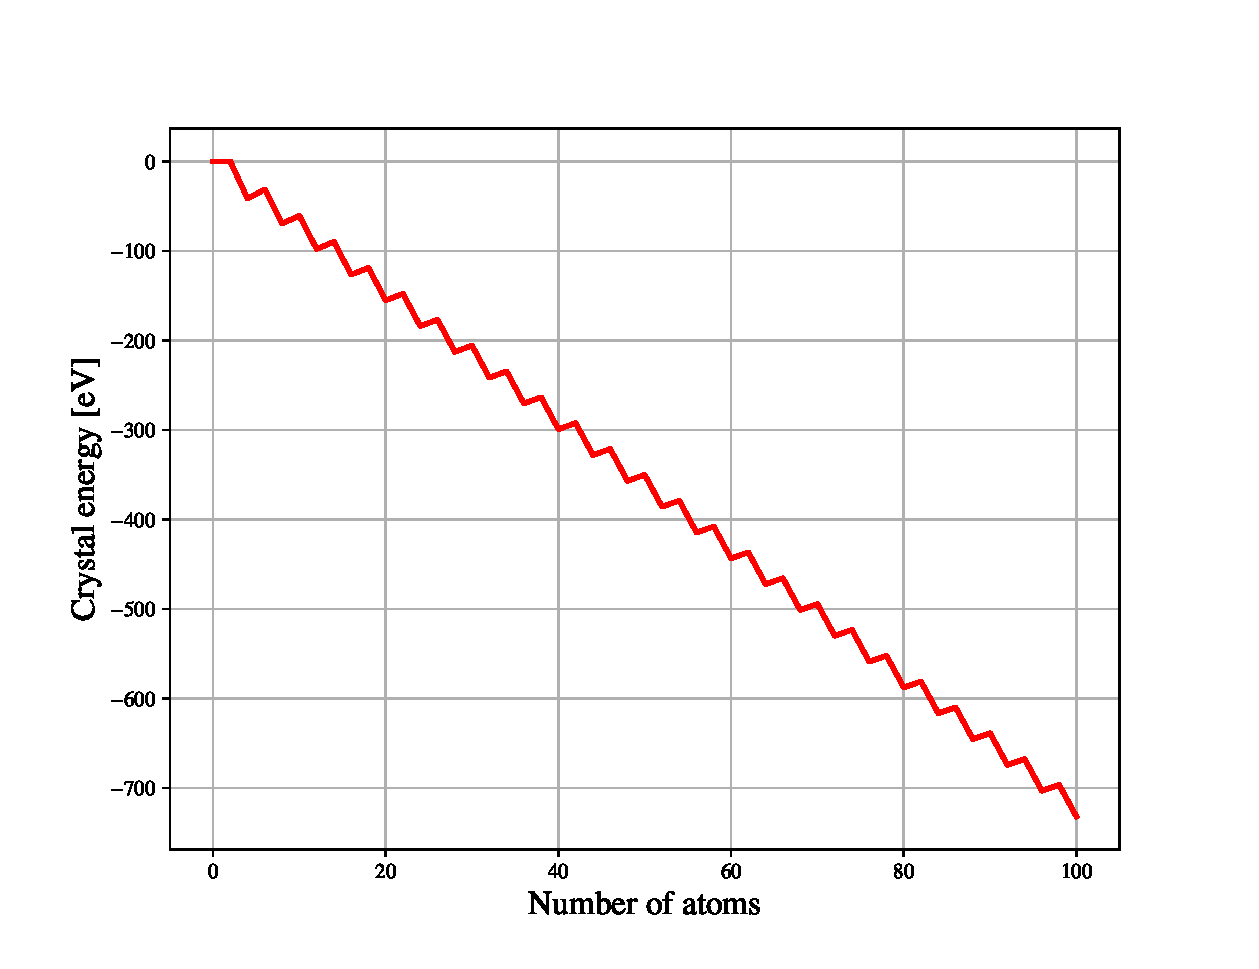
\includegraphics[scale=0.4]{figures/lattice_energy.eps}
    \captionof{figure}{Energy in the NaCl crystal as a function of the number of atoms}
    \label{fig:crystal_energy}
\end{minipage}
\begin{minipage}{.5\textwidth}
    \centering
    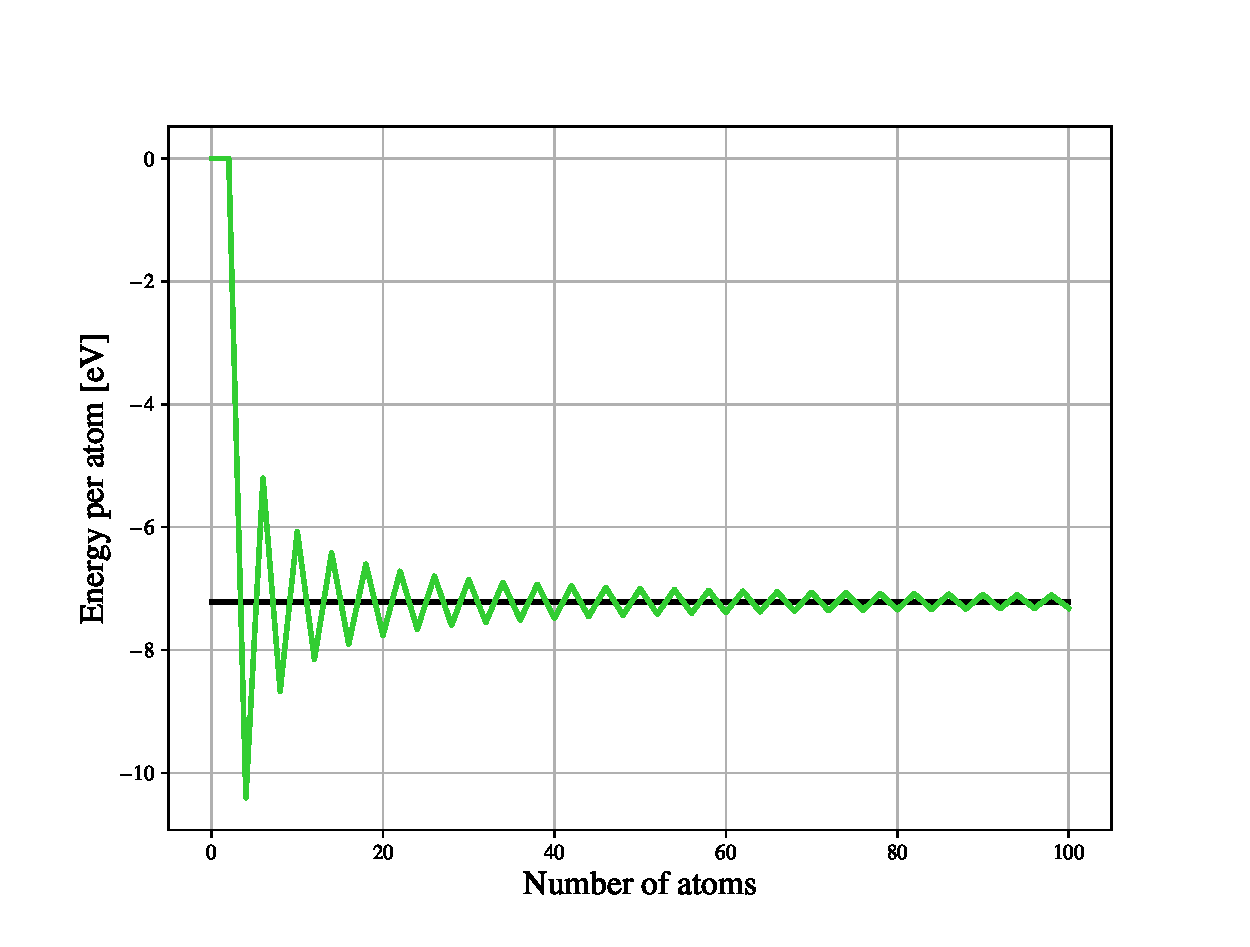
\includegraphics[scale=0.4]{figures/energy_per_atom.eps}
    \captionof{figure}{Energy per atom in the NaCl crystal as a function of the number of atoms (the Madelung constant changes)}
    \label{fig:energy_per_atom}
\end{minipage}
\end{figure}

\begin{figure}
    \centering 
    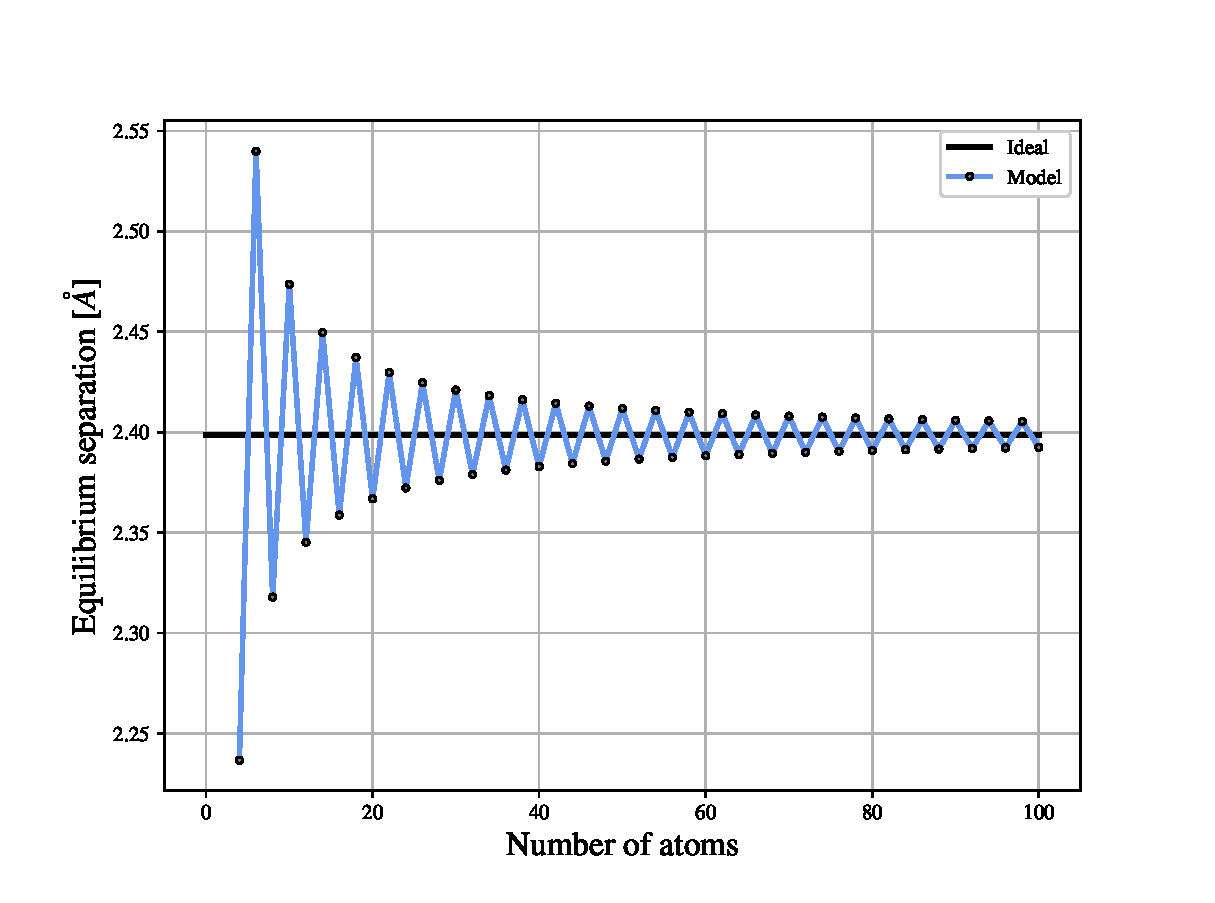
\includegraphics[scale=0.7]{figures/NaCl_constant.eps}
    \caption{Atoms' separation in the NaCl lattice as a function of the number of atoms in the crystal}
    \label{fig:NaCl_constant}
\end{figure}

\section*{Exercise 7}

\subsubsection*{(a)}
Suppose that we have N sites, and n of them are vacancies. Let us calculate the configurational entropy of the system as
$$S = k_B \ln\omega$$
If we imagine the sites as a 1D sequence we can calculate the number of microstates as the number of possible ways to 
combine $n$ objects of type $A$ with $N-n$ objects of type $B$
$$\omega(N, n) = \frac{N!}{n!(N-n)!}$$
Let us take the logarithm of this expression and use the Stirling's approximation
$$\ln \omega = \ln(N!) - \ln(n!) - \ln((N-n)!) \approx N \ln N - n \ln n - (N-n)\ln(N-n)$$
If temperature and pressure are constant, then the equilibrium state of the system is the one that minimizes the free energy
$$G = H - TS = U + pV - TS$$
In general the free energy of the system can be written as $G_{tot} = G_0(p, V, T, N) + \Delta G_{vac}(p, V, T, N, n)$, or,
in other words, I assume that the dependence of $G$ on the number of vacancies enters in the factor $\Delta G_{vac}$ (in principle $G_0$ could also be 0 at temperature T, I just want to underline that there might be another term that will be irrelevant for what follows). \\
We can search for the number of vacancies at equilibrium by imposing $$\frac{\partial G}{\partial n} = \frac{\partial \Delta G_{vac}}{\partial n} = 0$$
If we assume pressure and temperature constant we can write the free energy contribution due to the vacancies as
$$\Delta G = nE_f + n\sigma V_f- T\Delta S$$ 
where $E_f$ is the energy required to remove an atom from a site, $V_f$ is the formation volume and $\sigma$ is the modulus of the applied stress. Here I assumed that the formation energy and formation volume are the same for each atom 
and do not vary for successive extractions (at least approximately). The equation for the minimum becomes
$$ 0 = \frac{\partial \Delta G}{\partial n} = E_f + \sigma V_f + k_BT\ln\left(\frac{N-n}{n}\right)$$
and rearrangin terms
$$\frac{E_f + \sigma V}{k_BT} = -\ln\left(\frac{N-n}{n}\right)$$
or
$$\frac{n}{N-n} = \exp\left(-\frac{E_f}{k_B T}\right) \, \exp\left(-\frac{\sigma V_f}{k_B T}\right)$$
and if $n << N$
\begin{equation}
    c_v \simeq \frac{n}{N} = e^{-E_f/k_B T} \, e^{-\sigma V/k_B T}
    \label{eq:concentration}
\end{equation}

\subsubsection*{(b)}
The formation energy is the energy required to move an atom from the site to the surface of the lattice and in equation \ref{eq:concentration} is represented by $E_f$.
When an atom is removed the lattice get deformed and it generates an internal stress. The deformation causes a variation in the volume and the difference between the final state of the 
system (after moving the atom) and the initial state is the formation volume.

\newpage

\section*{Module II}

\subsection*{Exercise 2}
\begin{figure}
    \centering
    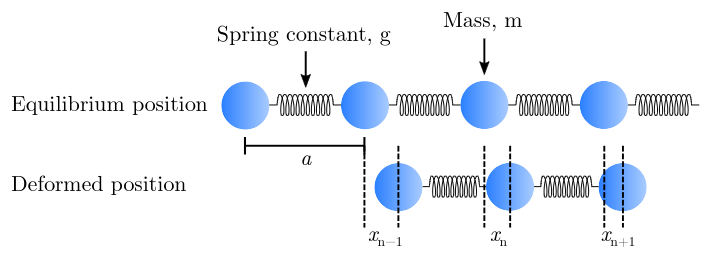
\includegraphics[scale=0.5]{figures/lattice_model.png}
    \caption{Model for the lattice vibrations}
    \label{fig:lattice_model}
\end{figure}
\subsubsection*{(a)}
Let us consider a chain of $N$ atoms as in figure \ref{fig:lattice_model}. The displacement of $n$-th from its equilibrium position is described by a function of the type
\begin{equation*}
    u_n(t) = u_n(0) \exp(i\omega t) \exp(inka)
\end{equation*}
Let us impose the Born-von Karman periodic boundary conditions on the lattice
\begin{equation*}
    u_n(t) = u_{n+N}(t)
\end{equation*}
which means
\begin{equation*}
    \exp(iNka) = 1
\end{equation*}
hence we find a condition on $k$
\begin{equation*}
    k = \frac{2n\pi}{N a}
\end{equation*}
This expressions indicates that the only vectors allowed with these boundary conditions are integer multiples of $\Delta k \equiv \frac{2\pi}{Na}$. The quantity $\Delta k$ is known as the 
wavevectors separation and indicates the space (in the $k$-space) between two different allowed wavevectors and represents the "required increment" of k to increase the number of phonons by one. 
This allows us to express the number of phonons in the crystal as a function of $k$ as 
\begin{equation}
    N(k) = \frac{k}{\Delta k} = \frac{kNa}{2\pi}
    \label{eq:number_modes}
\end{equation}
The phonons' density of states is defined as the number of phonons $dN = \frac{dN}{dk} dk$ contained in an interval $dk$ and from expression \ref{eq:number_modes} we see that
\begin{equation*}
    DOS(k) = \frac{dN(k)}{k} \, dk = \frac{Na}{2\pi}
\end{equation*}
\subsubsection*{(b)}
The given dispersion relation allows us to immediately calculate the density of states as a function of $\omega$ as
\begin{equation*}
    DOS(\omega) = \frac{dN}{d\omega} = \frac{dN}{dk}\frac{dk}{d\omega} = \frac{N}{\pi \omega_0} \frac{1}{\sqrt{1 - \omega/\omega_0}}
\end{equation*}

\section*{Exercise 4}
\begin{figure}[ht]
    \centering
      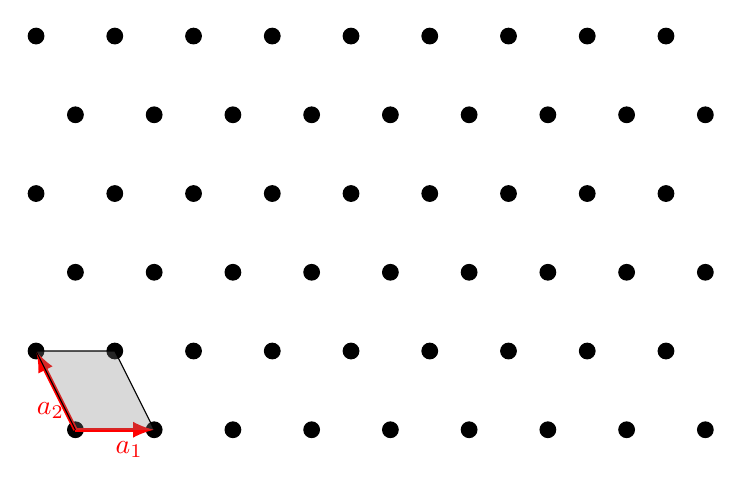
\begin{tikzpicture} 
          \foreach \y in {0,2,4}{
              \foreach \x in {1, 2, 3, 4, 5, 6, 7, 8, 9}{
                  \node[draw, circle, inner sep=2pt, fill] at (\x,\y){};
              }
          }
          \foreach \y in {1,3,5}{
              \foreach \x in {0.5, 1.5, 2.5, 3.5, 4.5, 5.5, 6.5, 7.5, 8.5}{
                  \node[draw, circle, inner sep=2pt, fill] at (\x,\y){};
              }
          }
          \draw [ultra thick, -latex, red] (1, 0) -- (2, 0) node [below left] {$a_1$};
          \draw [ultra thick, -latex, red]  (1, 0) node [above left] {$a_2$} -- (0.5, 1) ;
          \filldraw[fill=gray, fill opacity=0.3, draw=black] (1,0) -- (0.5,1) -- (1.5,1) -- (2,0);
          
      \end{tikzpicture}   
    \caption{lattice}
    \label{fig:hex}  
  \end{figure}
  %Draw reciprocal lattice
  \begin{figure}[ht]
    \centering
      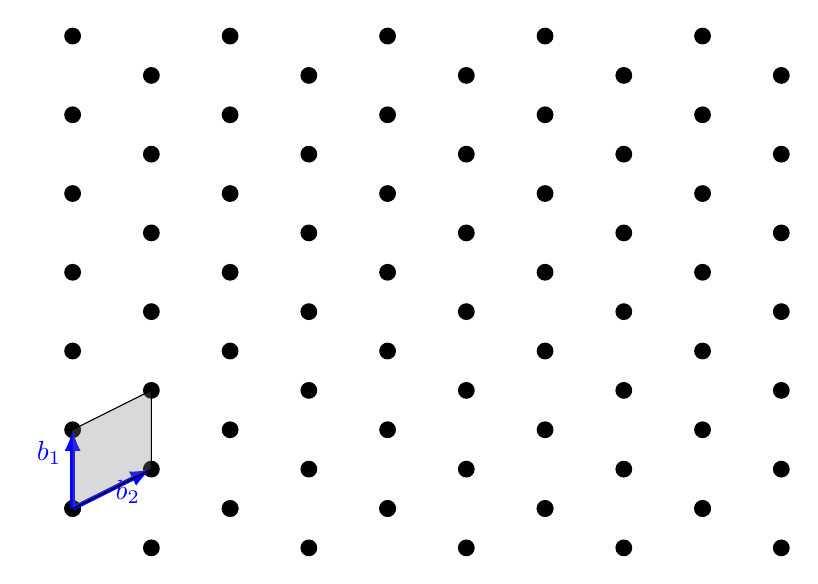
\begin{tikzpicture} 
          \foreach \x in {0,2,4,6,8}{
              \foreach \y in {1, 2, 3, 4, 5, 6, 7,}{
                  \node[draw, circle, inner sep=2pt, fill] at (\x,\y){};
              }
          }
          \foreach \x in {1,3,5,7,9}{
              \foreach \y in {0.5, 1.5, 2.5, 3.5, 4.5, 5.5, 6.5}{
                  \node[draw, circle, inner sep=2pt, fill] at (\x,\y){};
              }
          }
          \draw [ultra thick, -latex, blue] (0, 1) -- (0, 2) node [below left] {$b_1$};
          \draw [ultra thick, -latex, blue]  (0, 1) --  (1, 1.5) node [below left] {$b_2$} ;
          \filldraw[fill=gray, fill opacity=0.3, draw=black] (0,1) -- (1,1.5) -- (1,2.5) -- (0,2);
          
      \end{tikzpicture}   
    \caption{Reciprocal lattice}
    \label{fig:hex rep}  
  \end{figure}
Let us consider a general wave in the crystal
\begin{equation*}
    x_{u,v}(t) = u(0)\exp(-i\omega t)\exp(suk_1a)\exp(svk_2a)
\end{equation*}
Let us suppose that the last atom in the $\ve e_1$'s direction has coordinates $(N_xa,0)$ and the last one along $\ve e_2$ has coordinates $(0, N_ya)$ and let us suppose that $N_x=N_y$.
The boundary conditions are formally the same of the 2D's rectangular lattice, that is 
\begin{gather*}
    x_{0,v} = x_{N_x,v} \\
    x_{u,0} = x_{u,N_y}
\end{gather*}
hence the modes in the crystals are described by wavevectors $\ve k = (k_1, k_2)$ whose admitted values are for both
$$k_{s} = s\frac{\pi}{L} = s\frac{\pi}{Na} \qquad s \in \mathbb{N}$$ 
where $N$ denotes the number of atoms in the crystal. The spacing (area) between two successive modes is the area
$\Delta k \equiv \frac{\sqrt{3}}{2} \frac{\pi^2}{L^2}$. The number of modes contained in a quarter of a circle of radius $k_0$ is given by 
\begin{equation}
    n(k < k_0) = \frac{1}{4} \frac{\pi k_0^2}{\Delta k} = \frac{k_0^2 L^2}{2\sqrt{3}\,\pi}
    \label{eq:k_less_than_k0}
\end{equation}
Let us introduce now the toal number of atoms $N$. In principle not all the atoms contibutes to the number of degrees of freedom of the crystal: the atoms at the surface
are kept fixed (we imposed the boundary condition) and do not contribute to the total degrees of freedom. However, if $N>>1$ we expect the number of atoms in the surface to be 
negligible compared to the total number of atoms and we can approximate the total number of degrees of freedom with $2N$.
Hence, by inverting equation \ref{eq:k_less_than_k0} we get the maximum allowed $k$ in the crysal, that is 
\begin{equation*}
    k_D^2 = k_{max}^2 = \frac{2 \sqrt{3} \pi}{L^2} \, 2N = \frac{4 \sqrt{3} \pi}{L^2} \, N
\end{equation*}
and using the Debye's dispersion relation $\omega = v \, k$
\begin{equation*}
    \omega_D^2 = v^2 \frac{4 \sqrt{3} \pi }{L^2} \, N = \frac{4 \sqrt{3} \pi }{N a^2} \, v^2 
\end{equation*}
so that the Debye's frequency is 
\begin{equation*}
    \omega_D = \frac{2v}{a} \sqrt{\frac{\sqrt{3} \pi }{N}} \simeq 
\end{equation*}

\end{document}